\clearpage
\section{Bonus: Lasso and Relaxed Lasso}
\label{app:bonus_lasso}
This supplementary appendix documents the additional penalized classifiers fitted in the bonus section for the binary Jazz-versus-non-Jazz task.

For this binary classification problem, the lasso fit is a penalized logistic regression. Following Tibshirani~\cite{tibshirani1996lasso} and the binomial \texttt{glmnet} formulation described by Friedman, Hastie and Tibshirani~\cite{friedman2010glmnet}, the estimator solves
\begin{equation}
\hat{\beta}^{\mathrm{lasso}}(\lambda)=
\arg\min_{\beta_0,\beta}
\left\{
-\frac{1}{N}\sum_{i=1}^{N}\left[
y_i(\beta_0+x_i^\top\beta)-
\log\left(1+\exp(\beta_0+x_i^\top\beta)\right)
\right]
+\lambda\sum_{j=1}^{p}|\beta_j|
\right\},
\label{eq:bonus_lasso_logistic}
\end{equation}
so the fitting criterion combines the binomial negative log-likelihood with an \(\ell_1\) penalty. The role of this penalty is to shrink coefficients and to set some of them exactly to zero, which turns the estimation step into a variable-selection mechanism~\cite{tibshirani1996lasso,friedman2010glmnet}.

The active set selected by the lasso at a given value of \(\lambda\) is
\begin{equation}
M_{\lambda}=\left\{j \in \{1,\dots,p\}: \hat{\beta}^{\mathrm{lasso}}_j(\lambda)\neq 0\right\},
\label{eq:bonus_lasso_active_set}
\end{equation}
which is the notation used by Meinshausen~\cite{meinshausen2007relaxed} to define the relaxed lasso. The relaxed lasso keeps this support-selection step, but then reduces the amount of shrinkage applied after selection. In practical terms, it first identifies the subset \(M_{\lambda}\) with the ordinary lasso and then refits only the selected variables with a weaker penalty; at the strongest relaxation level, the selected support is effectively refit without penalization~\cite{meinshausen2007relaxed,hastie2020bestsubset}. This is why the relaxed lasso is often interpreted as a two-stage correction of the standard lasso: the first stage chooses the variables, and the second stage attenuates the bias induced by the \(\ell_1\) shrinkage.

\begin{figure}[H]
\centering
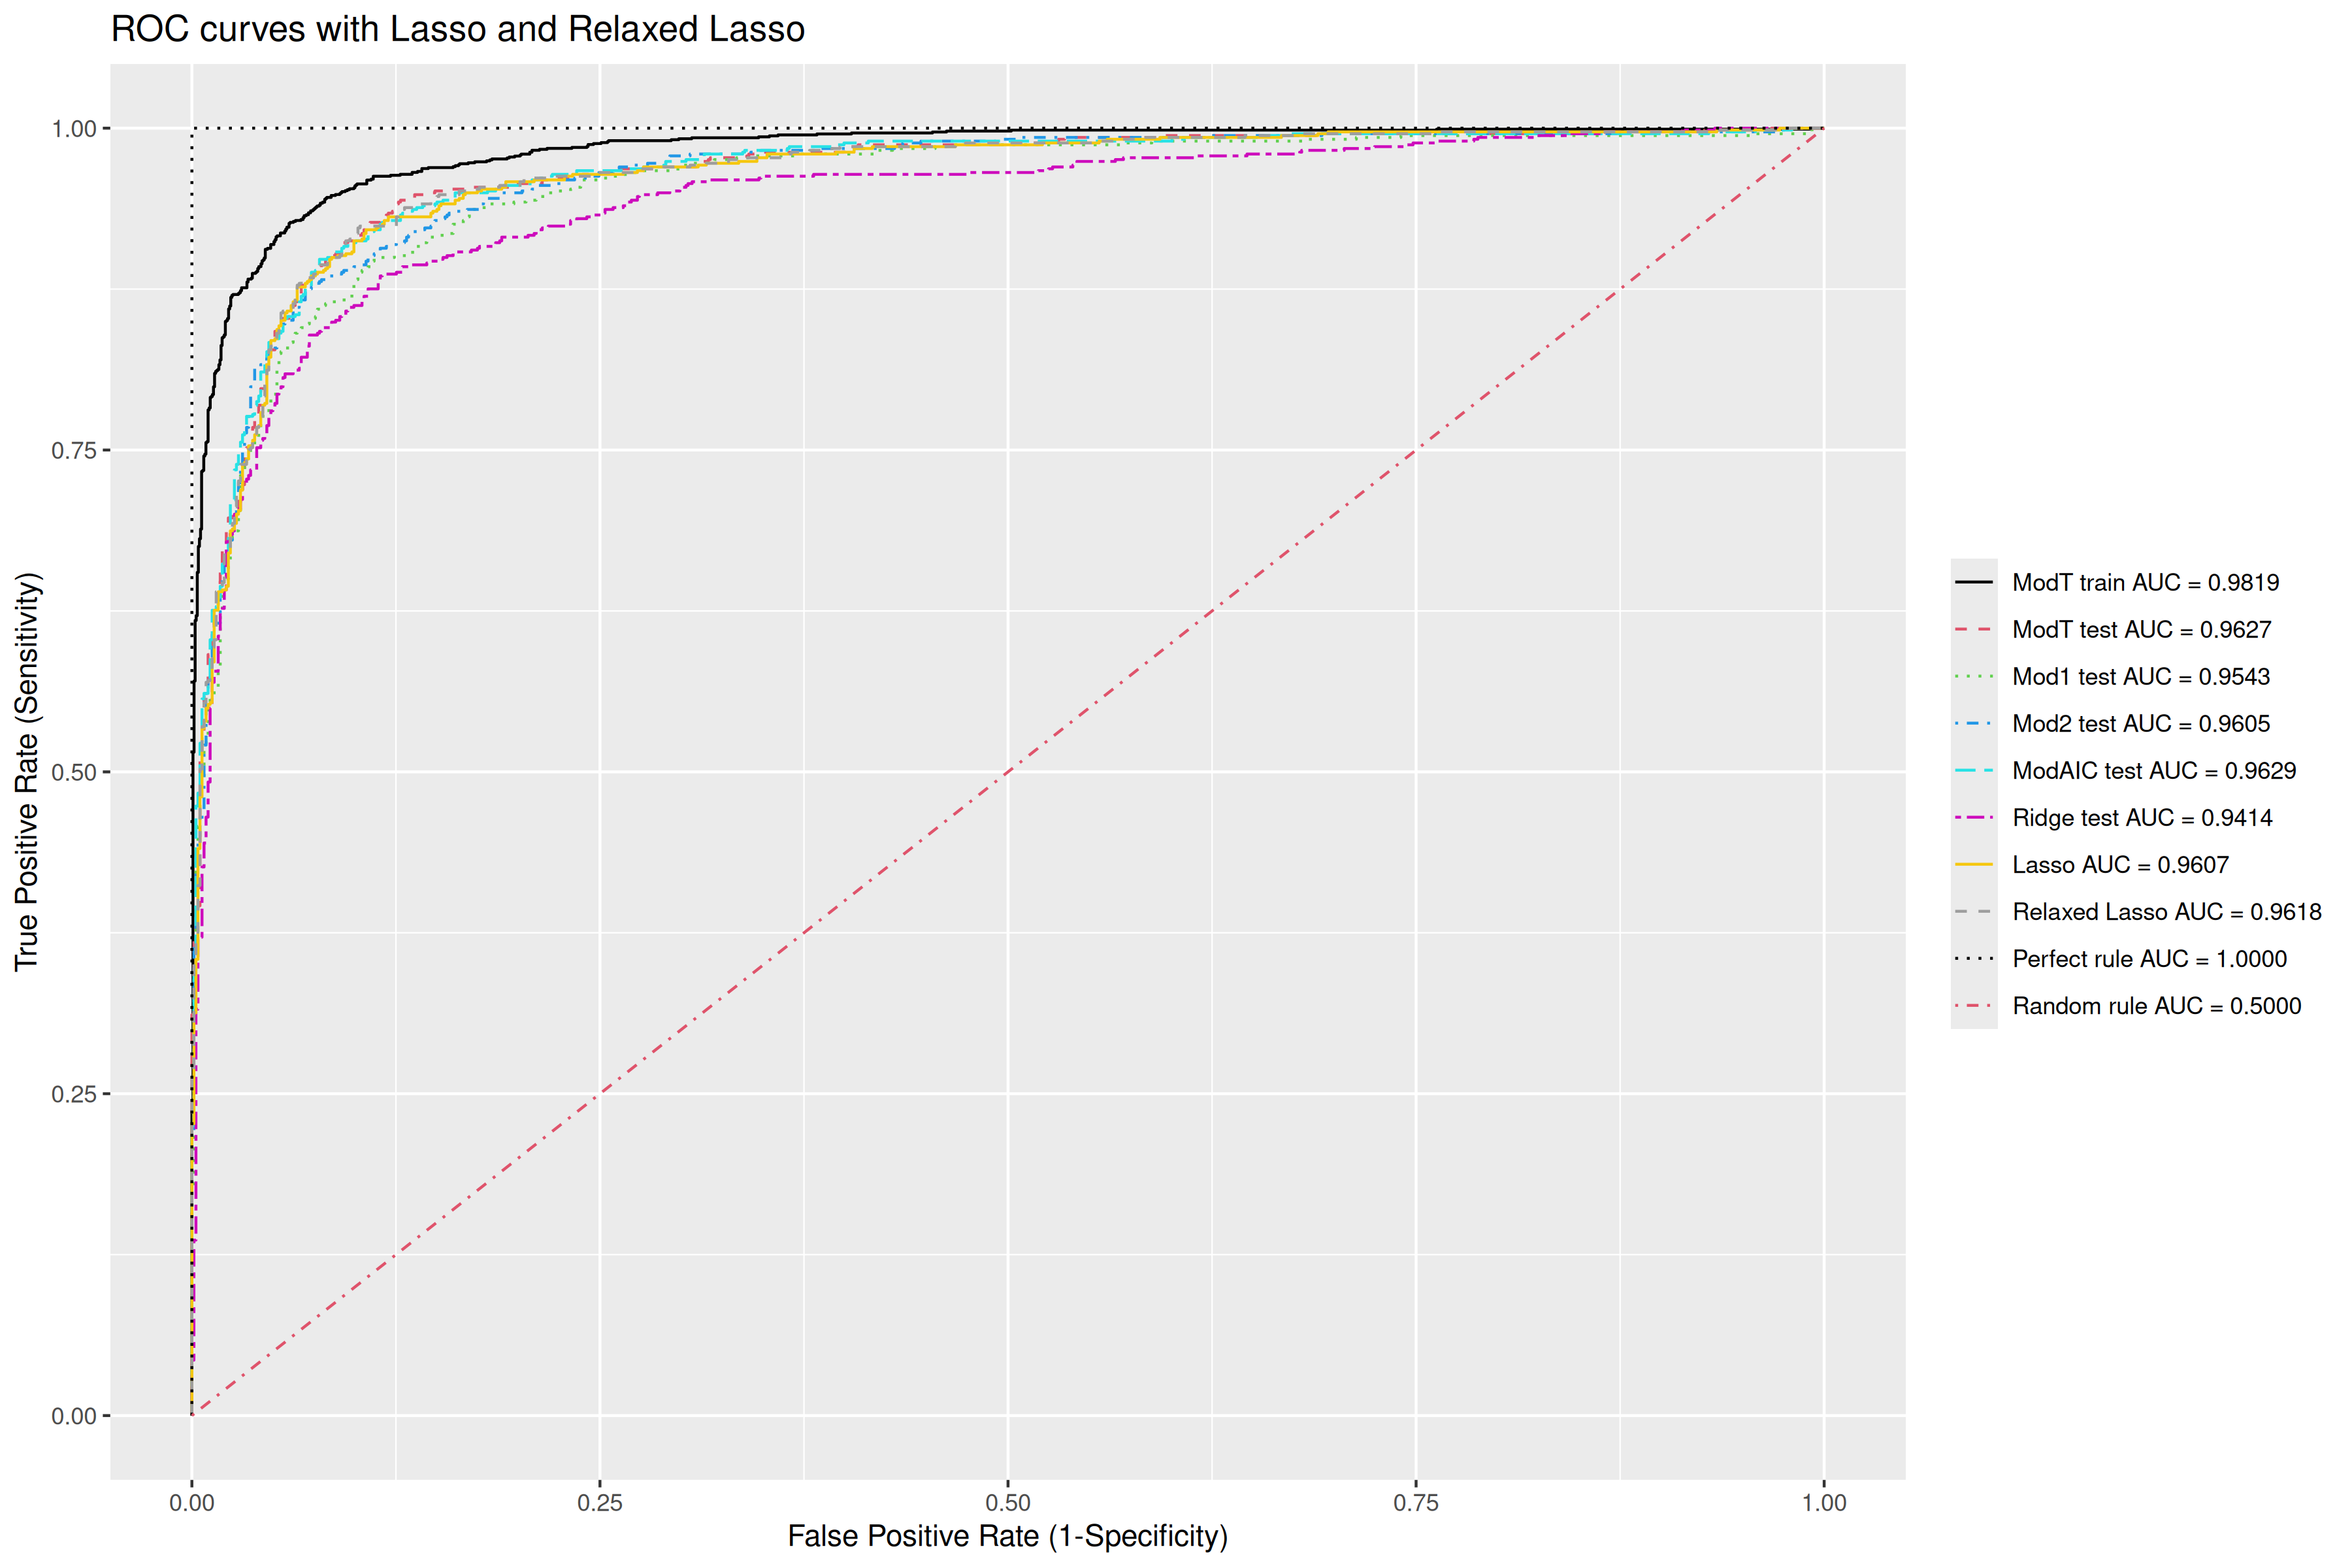
\includegraphics[width=0.9\columnwidth]{../output/part2/lasso/roc_curves_with_lasso.png}
\caption{ROC comparison after adding the Lasso and Relaxed Lasso bonus models to the binary benchmark.}
\label{fig:bonus_lasso_roc}
\end{figure}

From the AUC comparison, it can be observed that both the Lasso and relaxed Lasso models improve the test-set classification performance with respect to Ridge. This result is consistent with the nature of the Lasso penalty, since it not only reduces the magnitude of the coefficients but also performs variable selection. In a high-dimensional predictor space, this can remove noisy or weakly informative variables and lead to a more discriminative classifier. By contrast, Ridge keeps all predictors in the model, which may preserve less useful information and limit its predictive performance.

The results also show that relaxed Lasso improves over standard Lasso. This can be explained by the fact that relaxed Lasso preserves the subset of variables selected by the Lasso, but reduces the bias introduced by the \(L_1\) penalization on the selected coefficients. Consequently, it maintains the parsimony of the Lasso while recovering part of the discriminative capacity of the model, which can result in a higher AUC on the same test set.